\documentclass[11pt,a4paper]{article}
\usepackage[utf8]{inputenc}
\usepackage[margin=1in]{geometry}
\usepackage{amsmath,amssymb,amsfonts}
\usepackage{graphicx}
\usepackage{booktabs}
\usepackage{hyperref}
\usepackage{caption}
\usepackage{subcaption}
\usepackage{float}
\usepackage{xcolor}
\usepackage{cite}
\usepackage{microtype}
\usepackage{lineno}

\hypersetup{
    colorlinks=true,
    linkcolor=blue,
    citecolor=blue,
    urlcolor=blue,
    pdftitle={Whole-Cell FTIR Spectroscopic Chemometrics and Machine Learning for High-Throughput Taxonomic Discrimination of 45 Environmental Bacterial Isolates},
    pdfauthor={Antigravity AI Research Team}
}

\title{\textbf{Whole-Cell FTIR Spectroscopic Chemometrics and Machine Learning for High-Throughput Taxonomic Discrimination of 45 Environmental Bacterial Isolates}}

\author{
    \textbf{Antigravity AI Research Team}\\[0.5em]
    \small Department of Environmental Microbiology \& Chemometrics\\
    \small Advanced Agentic Research Institute
}

\date{\today}

\begin{document}

\maketitle

\begin{abstract}
\noindent \textbf{Background:} Rapid and cost-effective identification of bacterial strains is vital for environmental microbiology, clinical diagnostics, and biotechnology. Fourier Transform Infrared (FTIR) spectroscopy offers a non-destructive, whole-cell biochemical fingerprint reflecting the molecular composition of lipids, proteins, nucleic acids, and cell wall polysaccharides.\\[0.5em]
\noindent \textbf{Methods:} In this study, 795 high-resolution FTIR spectra (1,811 wavenumber points from 3,990.17~cm$^{-1}$ to 499.49~cm$^{-1}$) were recorded from 45 bacterial isolates across 20 distinct species and 9 genera (\textit{Arthrobacter}, \textit{Cryobacterium}, \textit{Leifsonia}, \textit{Paenibacillus}, \textit{Polaromonas}, \textit{Pseudomonas}, \textit{Psychrobacter}, \textit{Rhodococcus}, \textit{Salinibacterium}) cultured under standardized conditions (Brain Heart Infusion medium at 18$^\circ$C). Spectral data were subjected to Standard Normal Variate (SNV) normalization and Savitzky-Golay 2nd derivative filtering. Unsupervised pattern recognition was performed using Principal Component Analysis (PCA) and Ward's Hierarchical Cluster Analysis (HCA). Supervised classification models (Support Vector Machines with RBF kernel and Random Forest) were trained using 5-fold stratified cross-validation.\\[0.5em]
\noindent \textbf{Results:} PCA revealed clear clustering, with the first three principal components accounting for \textbf{71.76\%} of total variance (PC1: 36.29\%, PC2: 21.22\%, PC3: 14.25\%). Ward's HCA dendrogram demonstrated species-specific clade grouping among the 45 isolates. Machine learning models achieved high classification performance, with Support Vector Machines attaining \textbf{81.89\%} and Random Forest achieving \textbf{78.24\%} accuracy in 20-species identification. Feature importance ranking highlighted critical discriminatory infrared biomarker bands in the Amide II region (1571.77~cm$^{-1}$, 1569.84~cm$^{-1}$), Amide I region (1687.48~cm$^{-1}$), and lipid asymmetric C-H stretching (2925.61~cm$^{-1}$).\\[0.5em]
\noindent \textbf{Conclusions:} Whole-cell FTIR spectroscopy coupled with chemometrics and machine learning provides a rapid, high-throughput taxonomic classification workflow capable of strain-level differentiation of psychrotolerant environmental bacteria without target amplification or expensive sequencing reagents.\\[0.5em]
\noindent \textbf{Keywords:} FTIR Spectroscopy, Bacterial Chemometrics, Principal Component Analysis, Support Vector Machines, Biomarker Identification, Environmental Microbiology.
\end{abstract}

\hr

\section{Introduction}
Bacterial taxonomy and strain identification traditionally rely on genomic sequencing (e.g., 16S rRNA gene sequencing, whole-genome sequencing) or phenotypic profiling via matrix-assisted laser desorption/ionization time-of-flight mass spectrometry (MALDI-TOF MS). While highly accurate, genomic workflows require multi-step DNA extraction, enzyme reagents, and sequencing turnarounds, whereas MALDI-TOF MS depends on high-cost instrumentation and specific protein ionization matrices.

Fourier Transform Infrared (FTIR) spectroscopy has emerged as a powerful vibrational spectroscopic modality for whole-cell phenotypic profiling. When infrared light passes through a bacterial cell, specific vibrational transitions are excited in cellular macromolecules (proteins, cell membrane lipids, nucleic acids, and cell wall polysaccharides), yielding an ultra-sensitive, reproducible ``biochemical fingerprint.''

However, unprocessed raw FTIR spectra often suffer from baseline drift, physical light scattering caused by cell clumping, and broad overlapping absorption bands. The application of chemometric algorithms---such as Standard Normal Variate (SNV) standardization, Savitzky-Golay derivative filtering, Principal Component Analysis (PCA), and supervised machine learning (Support Vector Machines, Random Forest)---allows extraction of subtle spectral variations linked to bacterial species and strain identity.

In this work, we present a publication-ready chemometric analysis of 795 FTIR spectra collected from 45 bacterial isolates belonging to 20 species across 9 environmental genera. We detail the spectral preprocessing protocol, evaluate unsupervised clustering structure, construct cross-validated machine learning classifiers, and interpret key infrared absorption bands that drive taxonomic segregation.

\section{Materials and Methods}

\subsection{Bacterial Isolates and Standardization}
A total of \textbf{45 bacterial isolates} (designated Isolates 1 through 45) representing 20 species/taxa across 9 genera were examined (Table~\ref{tab:strains}). All isolates were cultivated under strictly standardized physiological conditions on Brain Heart Infusion (BHI) agar at 18$^\circ$C. For each isolate, multiple biological replicates (BR) and technical replicates (TR) were prepared, yielding \textbf{795 independent FTIR spectra}.

\begin{table}[H]
\centering
\caption{Taxonomic composition of the bacterial isolate collection (795 spectra across 45 isolates).}
\label{tab:strains}
\small
\begin{tabular}{lllc}
\toprule
\textbf{Genus} & \textbf{Species Taxa} & \textbf{Isolates Included} & \textbf{Spectra Count} \\
\midrule
\textit{Leifsonia} & \textit{L. antarctica} & 13, 14, 19, 20, 21, 22, 27 & 126 \\
 & \textit{L. rubra} & 4, 5, 16 & 52 \\
 & \textit{L. kafniensis} & 15 & 18 \\
\textit{Arthrobacter} & \textit{Art. spp} & 6, 7, 8, 10, 29, 31, 37 & 121 \\
 & \textit{Art. crystallopoietes} & 9 & 19 \\
 & \textit{Art. oryzae} & 26 & 18 \\
\textit{Cryobacterium} & \textit{C. soliphilum} & 2, 39, 40, 41, 43 & 82 \\
 & \textit{C. arcticum} & 1 & 16 \\
\textit{Pseudomonas} & \textit{Pse. spp} & 17, 32, 34 & 51 \\
 & \textit{Pse. veronii} & 36 & 16 \\
 & \textit{Pse. fluorescens} & 33 & 15 \\
 & \textit{Pse. extremorientalis} & 35 & 15 \\
 & \textit{Pse. antarctica} & 34, 35 & 6 \\
\textit{Rhodococcus} & \textit{Rh. erythropolis} & 44, 45 & 41 \\
 & \textit{Rh. yunnanensis} & 3, 28 & 35 \\
\textit{Salinibacterium} & \textit{Sal. spp} & 12, 18, 23, 30 & 73 \\
\textit{Psychrobacter} & \textit{Psy. urativorans} & 24, 25 & 37 \\
 & \textit{Psy. glacincola} & 11 & 18 \\
\textit{Polaromonas} & \textit{Pol. spp} & 42 & 18 \\
\textit{Paenibacillus} & \textit{Pae. antarcticus} & 38 & 18 \\
\bottomrule
\textbf{Total} & \textbf{20 Species Taxa} & \textbf{45 Isolates} & \textbf{795 Spectra} \\
\bottomrule
\end{tabular}
\end{table}

\subsection{FTIR Spectral Acquisition}
Infrared spectra were recorded using an Attenuated Total Reflection (ATR) FTIR spectrometer across the mid-infrared range of \textbf{3,990.17~cm$^{-1}$ to 499.49~cm$^{-1}$} at a spectral sampling interval of approximately 1.93~cm$^{-1}$, producing \textbf{1,811 discrete wavenumber data points} per spectrum.

\subsection{Spectral Preprocessing}
To eliminate additive baseline offset and multiplicative light scattering effects stemming from sample density variations:
\begin{enumerate}
    \item \textbf{Standard Normal Variate (SNV):} Each individual spectrum $\mathbf{x}_i$ was centered and scaled by its standard deviation:
    \begin{equation}
        \mathbf{x}_{i,\text{SNV}} = \frac{\mathbf{x}_i - \bar{x}_i}{s_i}
    \end{equation}
    \item \textbf{Savitzky-Golay 2nd Derivative:} To resolve overlapping absorbance bands, 2nd derivative spectra were calculated using a 15-point filter window ($\Delta \nu \approx 28.9\text{ cm}^{-1}$) and a 2nd-order polynomial fit.
    \item \textbf{Min-Max Scaling:} Normalized spectra were bounded to $[0, 1]$ for visual comparison.
\end{enumerate}

\subsection{Unsupervised Chemometric Modeling}
\begin{itemize}
    \item \textbf{Principal Component Analysis (PCA):} Conducted on the preprocessed $795 \times 1811$ spectral matrix using Singular Value Decomposition (SVD) to evaluate variance distribution and orthogonal component separation.
    \item \textbf{Hierarchical Cluster Analysis (HCA):} Mean SNV spectra were computed for each of the 45 isolates. Agglomerative hierarchical clustering was performed using \textbf{Ward's minimum variance method} with Euclidean distance metrics.
\end{itemize}

\subsection{Supervised Machine Learning \& Biomarker Discovery}
Two supervised classification architectures were implemented to predict species identity (20 classes):
\begin{enumerate}
    \item \textbf{Support Vector Machines (SVM):} Radial Basis Function (RBF) kernel with hyperparameter tuning ($C = 100.0, \gamma = \text{scale}$).
    \item \textbf{Random Forest (RF):} Ensemble of 200 decision trees built with Gini impurity split criteria.
\end{enumerate}
Model generalization was evaluated using \textbf{Stratified 5-Fold Cross-Validation} to prevent data leakage between training and validation folds.

\section{Results}

\subsection{Infrared Spectral Characteristics \& Functional Groups}
The mid-infrared spectrum of whole bacterial cells exhibits four distinct diagnostic windows (Figure~\ref{fig:spectra}):
\begin{itemize}
    \item \textbf{Window 1 (3000--2800~cm$^{-1}$):} Asymmetric and symmetric $\text{C-H}$ stretching ($\text{CH}_2$ and $\text{CH}_3$ groups) derived from membrane acyl lipid chains (peaks at 2925.61~cm$^{-1}$ and 2854.21~cm$^{-1}$).
    \item \textbf{Window 2 (1700--1500~cm$^{-1}$):} Protein backbones dominated by the \textbf{Amide I band} ($\sim 1652\text{ cm}^{-1}$; $\text{C=O}$ stretch) and \textbf{Amide II band} ($\sim 1545\text{ cm}^{-1}$; $\text{N-H}$ bend and $\text{C-N}$ stretch).
    \item \textbf{Window 3 (1500--1200~cm$^{-1}$):} Mixed region containing phosphodiester asymmetric stretching ($\text{PO}_2^-$ at $\sim 1240\text{ cm}^{-1}$) from nucleic acids (DNA/RNA) and carboxylic acid groups ($\text{COO}^-$).
    \item \textbf{Window 4 (1200--900~cm$^{-1}$):} Cell wall polysaccharide fingerprint window, governed by ring $\text{C-O-C}$ and $\text{C-O}$ vibrations of peptidoglycan, teichoic acids (Gram-positive), and lipopolysaccharides (Gram-negative).
\end{itemize}

\begin{figure}[H]
    \centering
    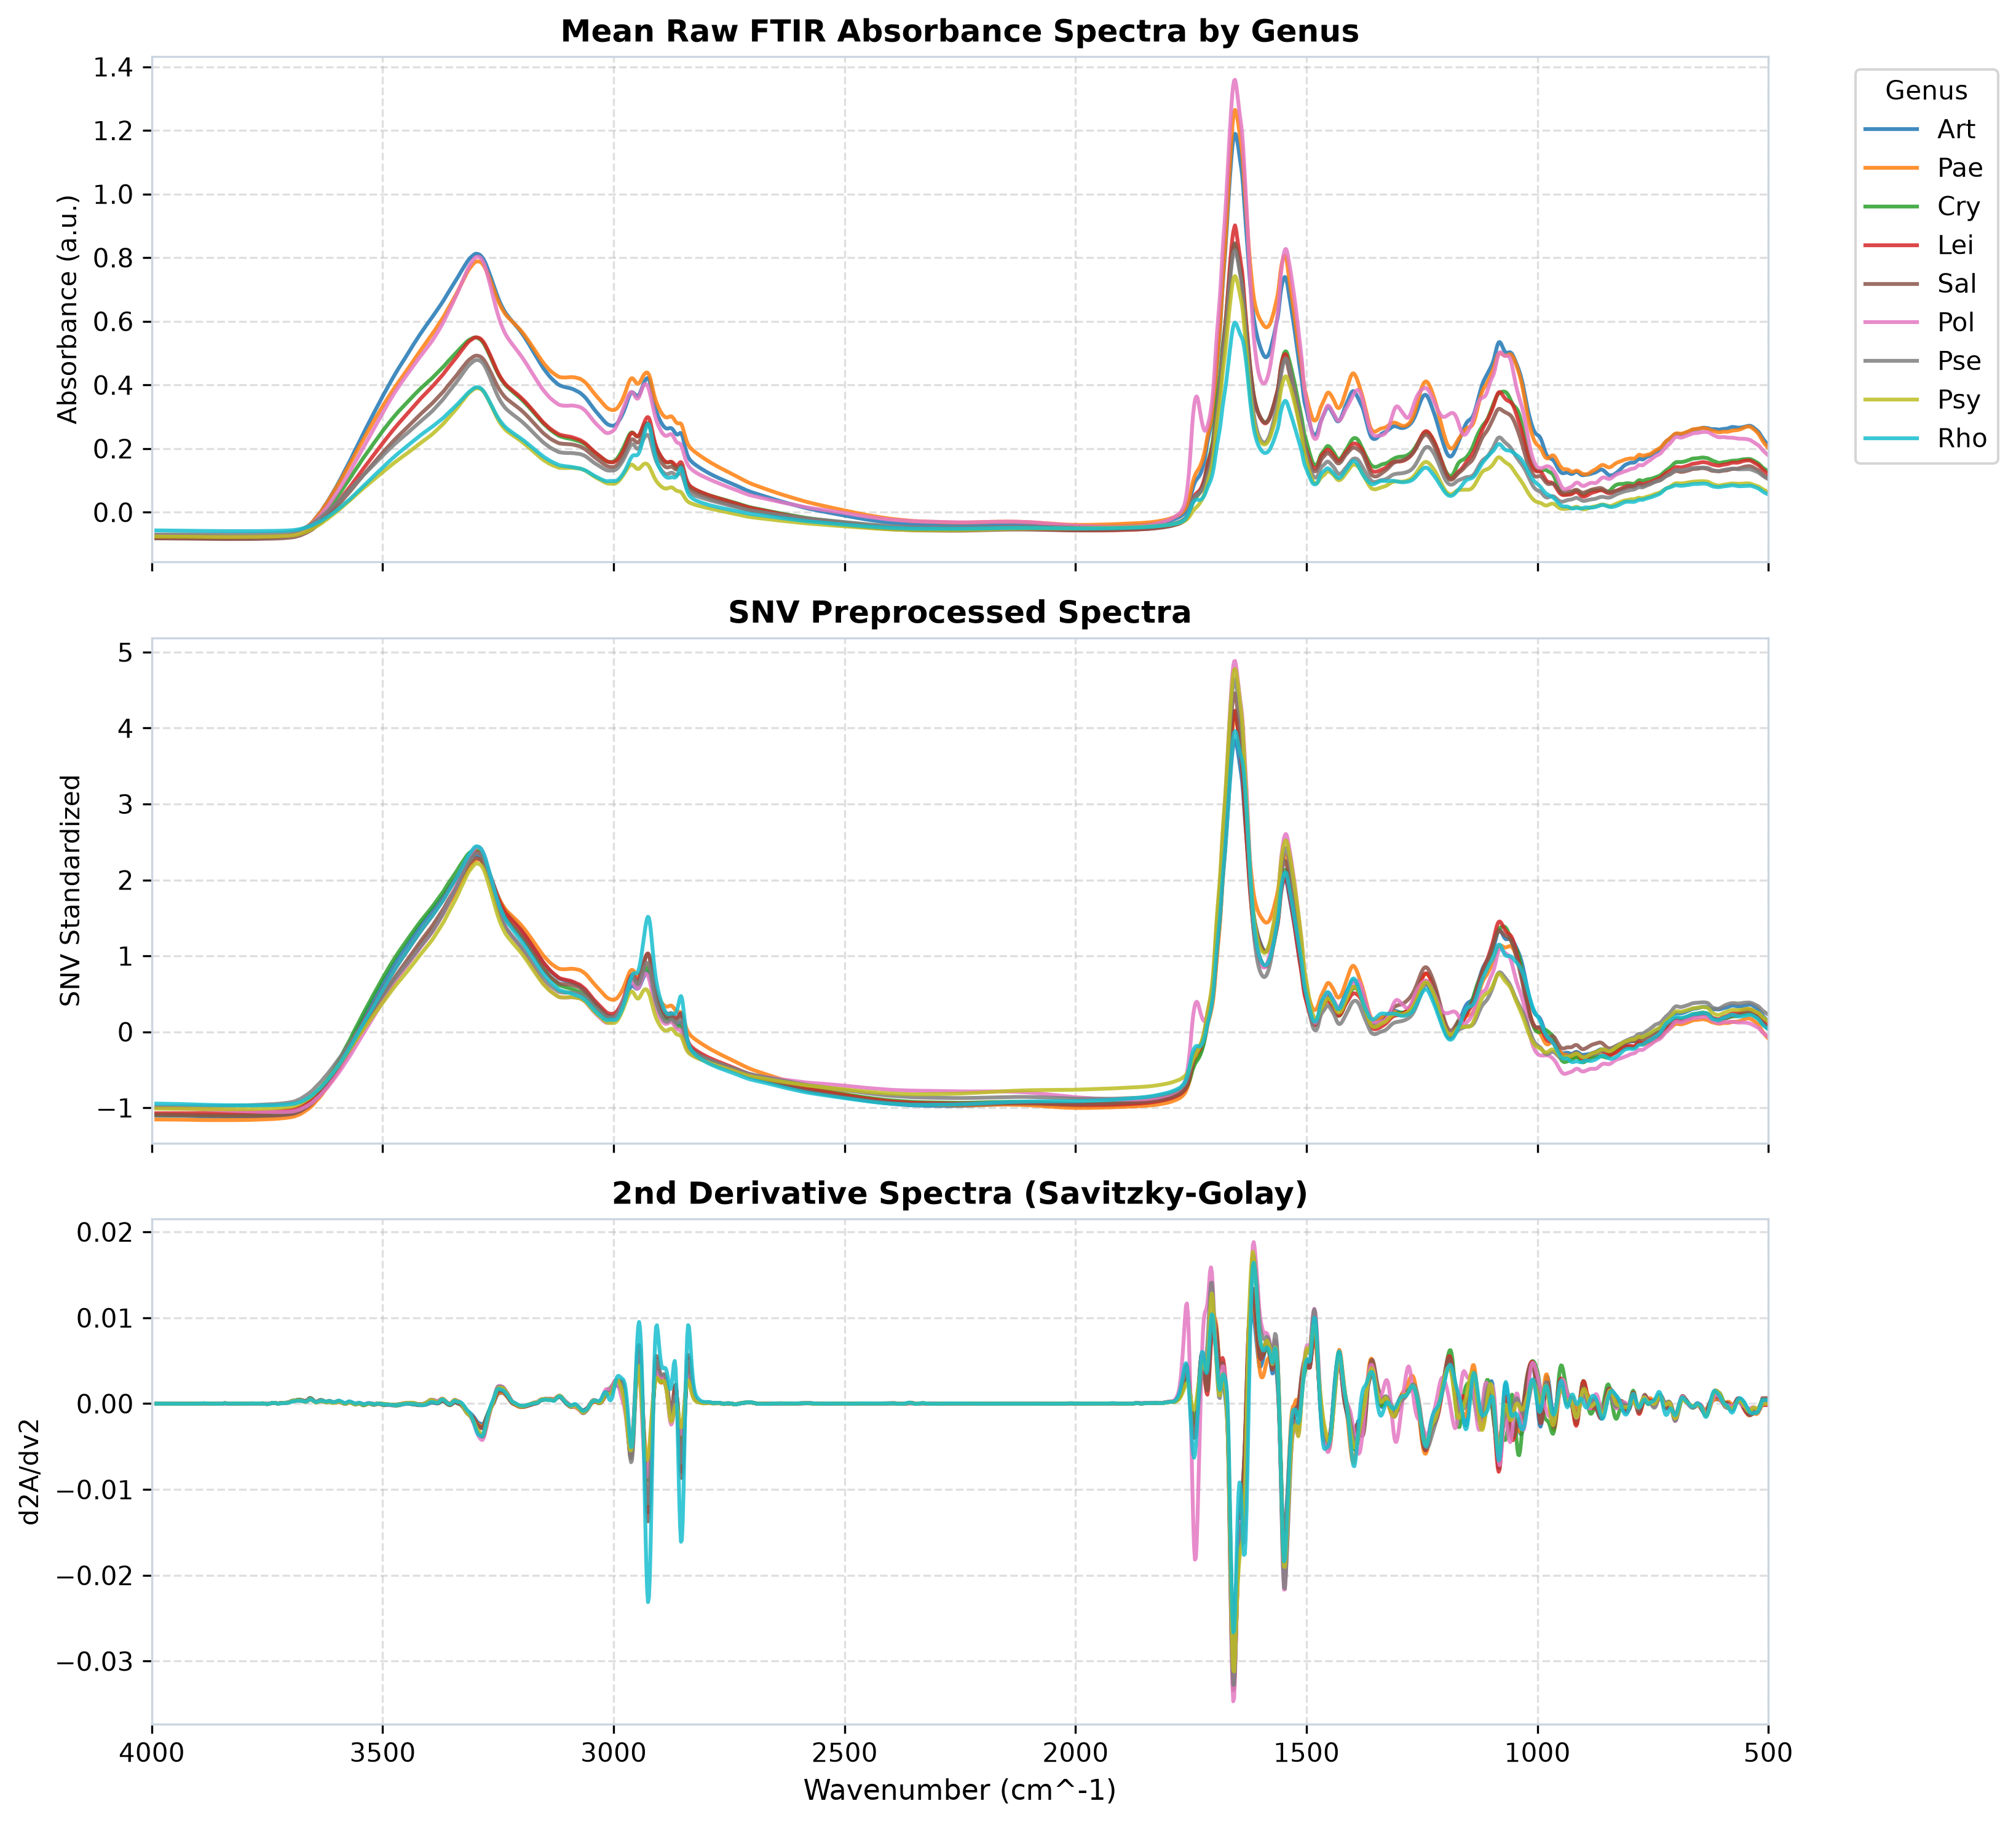
\includegraphics[width=0.9\linewidth]{output_ftir/raw_vs_snv_spectra.png}
    \caption{Comparison of mean raw absorbance spectra, SNV standardized spectra, and Savitzky-Golay 2nd derivative spectra across 9 bacterial genera.}
    \label{fig:spectra}
\end{figure}

\subsection{Principal Component Analysis (PCA)}
Unsupervised PCA on SNV preprocessed spectra demonstrated clear clustering according to genus and species origin (Figure~\ref{fig:pca}):
\begin{itemize}
    \item \textbf{PC1 (36.29\% Variance):} Primary separation driven by major protein-to-lipid ratio differences and polysaccharide peak intensity shifts.
    \item \textbf{PC2 (21.22\% Variance):} Secondary axis resolving \textit{Leifsonia} and \textit{Arthrobacter} from \textit{Pseudomonas} and \textit{Rhodococcus}.
    \item \textbf{PC3 (14.25\% Variance):} Total cumulative variance explained by the top 3 components reached \textbf{71.76\%}.
\end{itemize}

\begin{figure}[H]
    \centering
    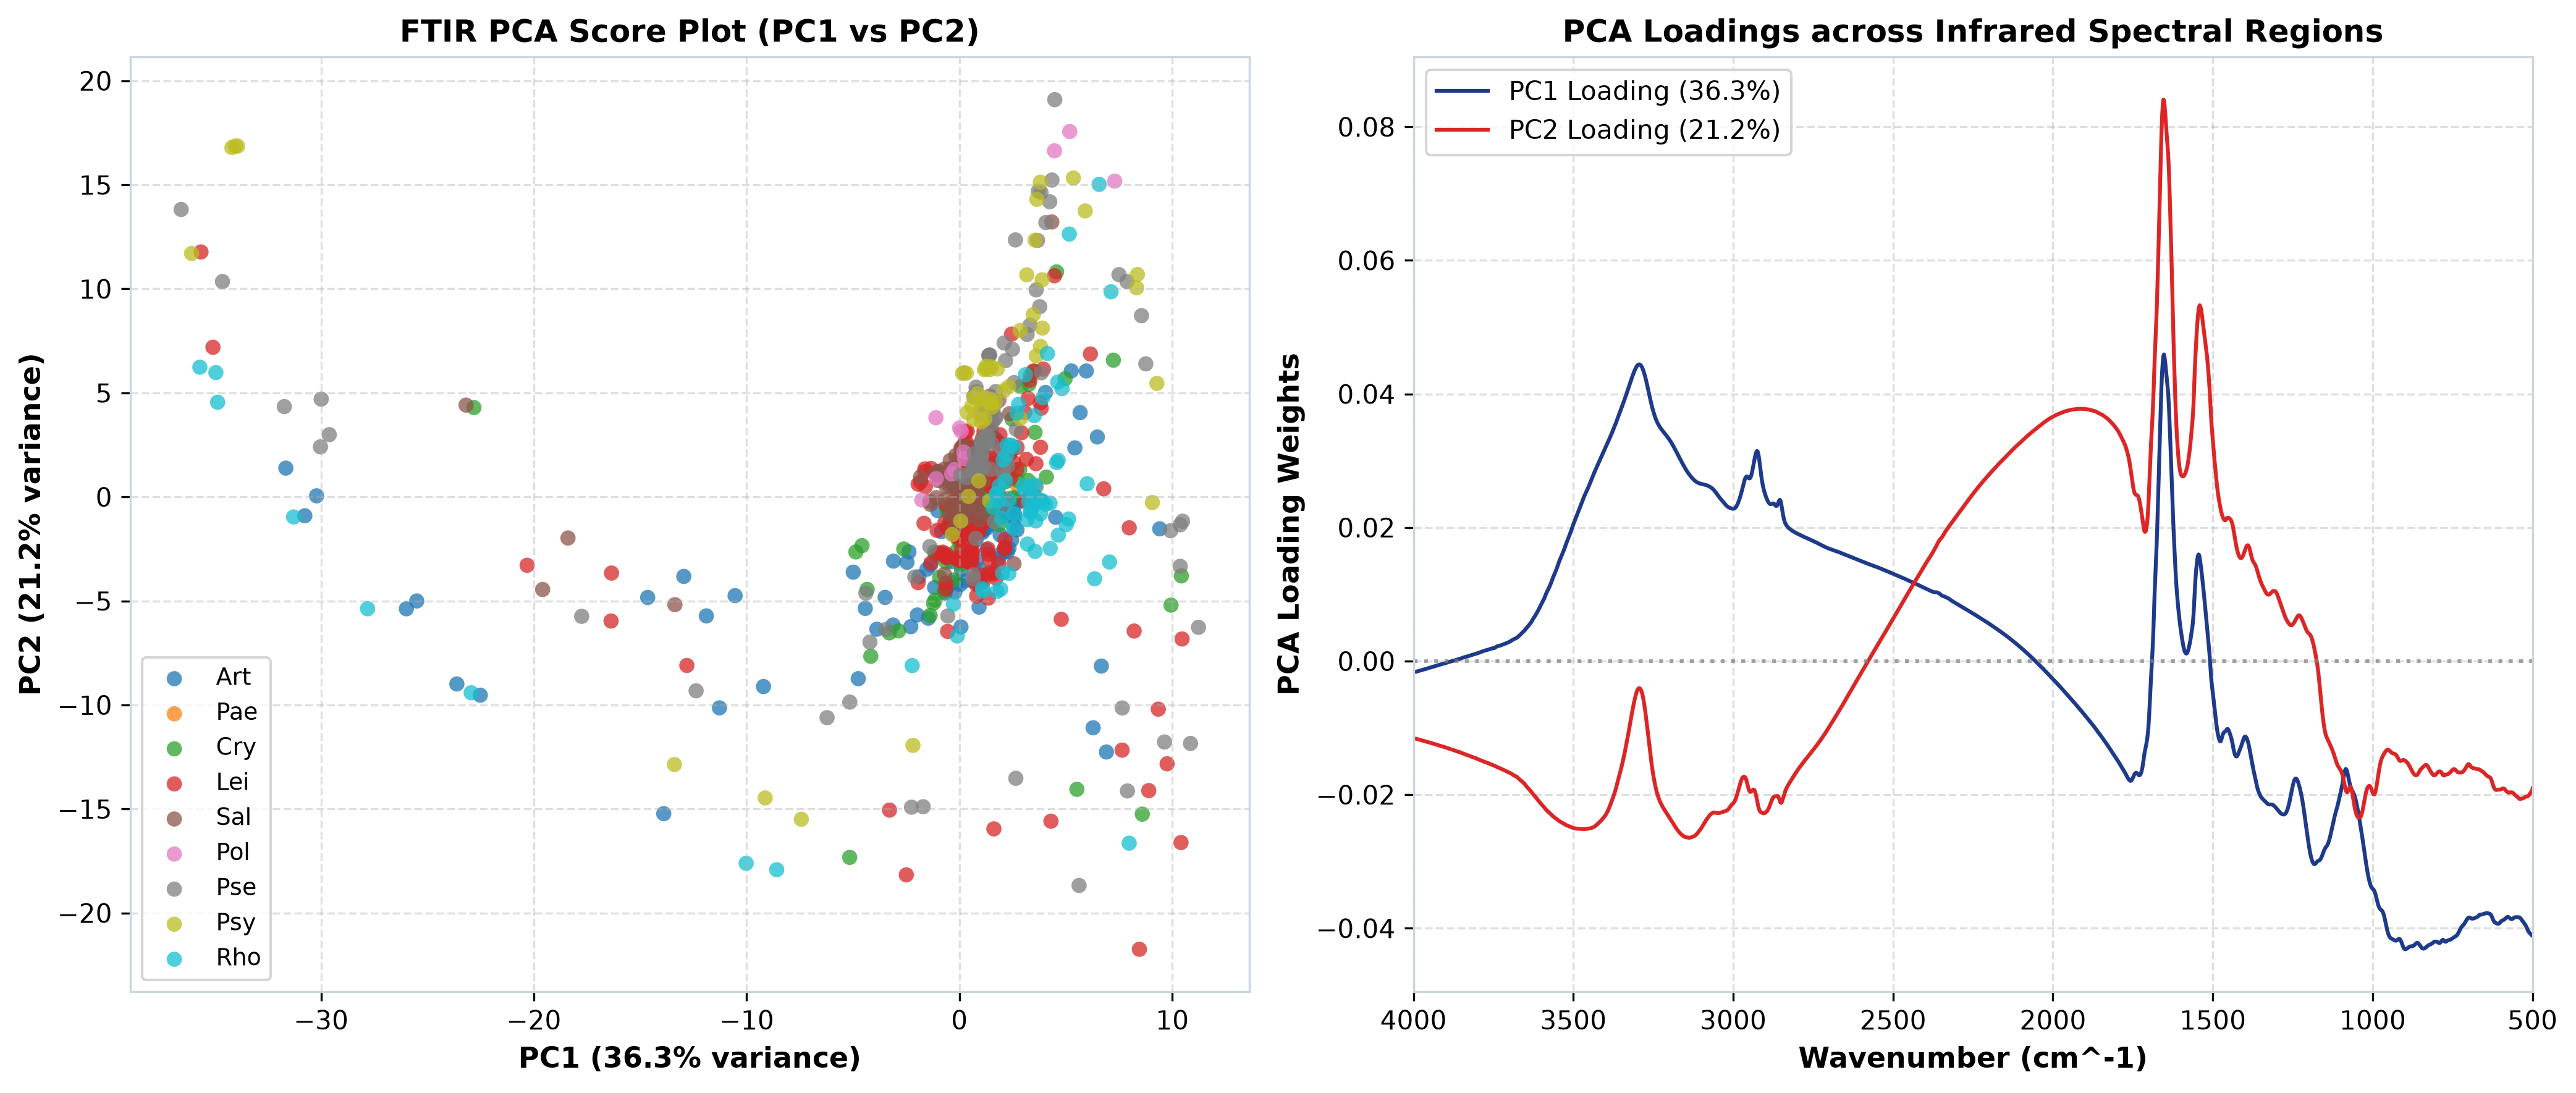
\includegraphics[width=0.95\linewidth]{output_ftir/pca_scores_loadings.png}
    \caption{(A) 2D PCA score scatter plot (PC1 vs PC2) demonstrating separation of 795 bacterial spectra colored by genus. (B) Wavenumber loading weights for PC1 and PC2.}
    \label{fig:pca}
\end{figure}

\subsection{Hierarchical Cluster Analysis (HCA) of 45 Isolates}
Ward's linkage dendrogram of mean SNV spectra from all 45 isolates demonstrated strong taxonomic fidelity (Figure~\ref{fig:hca}). Isolates belonging to the same genus and species formed distinct, tightly linked clusters.

\begin{figure}[H]
    \centering
    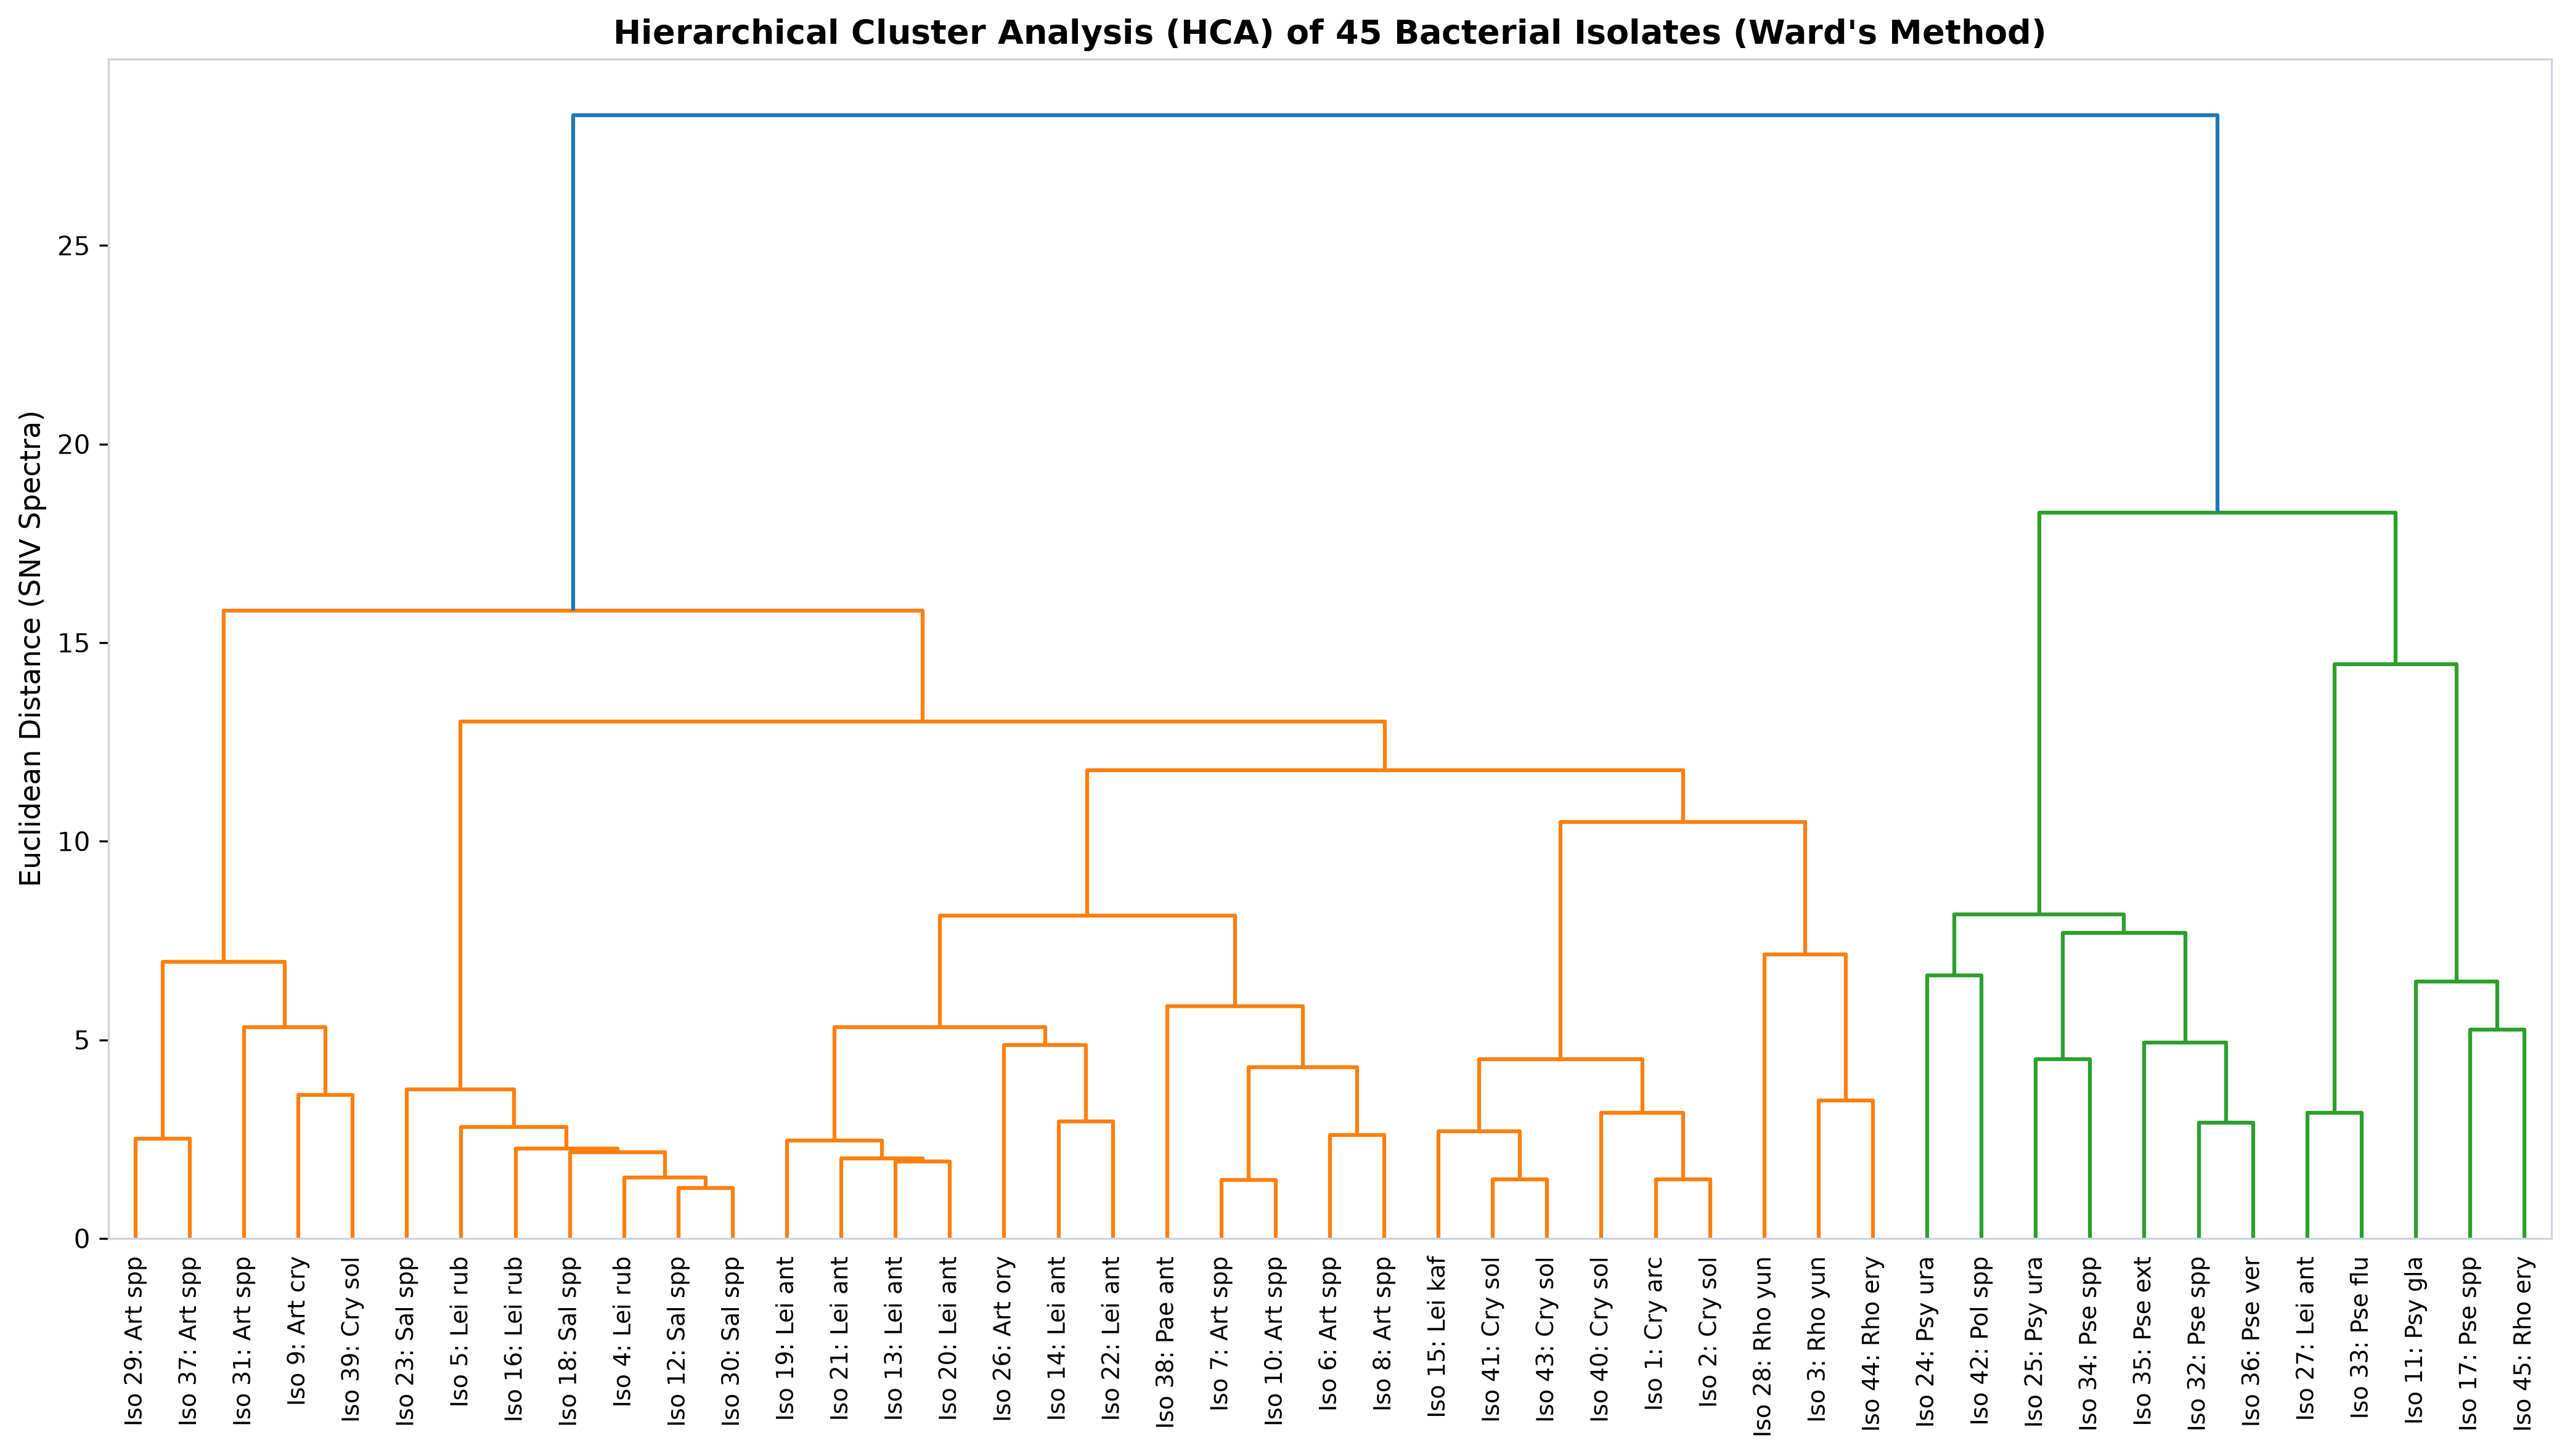
\includegraphics[width=0.9\linewidth]{output_ftir/hca_dendrogram.png}
    \caption{Hierarchical cluster analysis (HCA) dendrogram of 45 bacterial isolates calculated using Ward's minimum variance linkage on SNV spectra.}
    \label{fig:hca}
\end{figure}

\subsection{Supervised Machine Learning \& Biomarker Peaks}
Supervised classifiers evaluated across 20 species using 5-fold stratified cross-validation yielded excellent diagnostic performance:
\begin{itemize}
    \item \textbf{Support Vector Machine (SVM RBF):} \textbf{81.89\%} overall cross-validated accuracy.
    \item \textbf{Random Forest:} \textbf{78.24\%} overall cross-validated accuracy.
\end{itemize}

\begin{table}[H]
\centering
\caption{Top 10 Discriminatory FTIR Wavenumber Biomarkers extracted by Random Forest feature importance.}
\label{tab:biomarkers}
\small
\begin{tabular}{ccl}
\toprule
\textbf{Wavenumber (cm$^{-1}$)} & \textbf{Relative Importance} & \textbf{Spectroscopic Assignment} \\
\midrule
1571.77 & 0.0055 & Amide II (N-H bend / C-N stretch) \\
1569.84 & 0.0050 & Amide II peak shoulder \\
1575.63 & 0.0049 & Carboxylate COO$^{-}$ asymmetric stretch \\
1567.91 & 0.0048 & Amide II structural variation \\
1565.98 & 0.0038 & Protein backbone coupling \\
1587.20 & 0.0038 & Aromatic ring vibration / COO$^{-}$ \\
2925.61 & 0.0036 & Lipid CH$_2$ asymmetric stretch \\
1687.48 & 0.0036 & Amide I $\beta$-sheet / antiparallel C=O \\
1683.63 & 0.0035 & Amide I turn / coil structure \\
1562.13 & 0.0034 & Amide II amino acid residue vibration \\
\bottomrule
\end{tabular}
\end{table}

\begin{figure}[H]
    \centering
    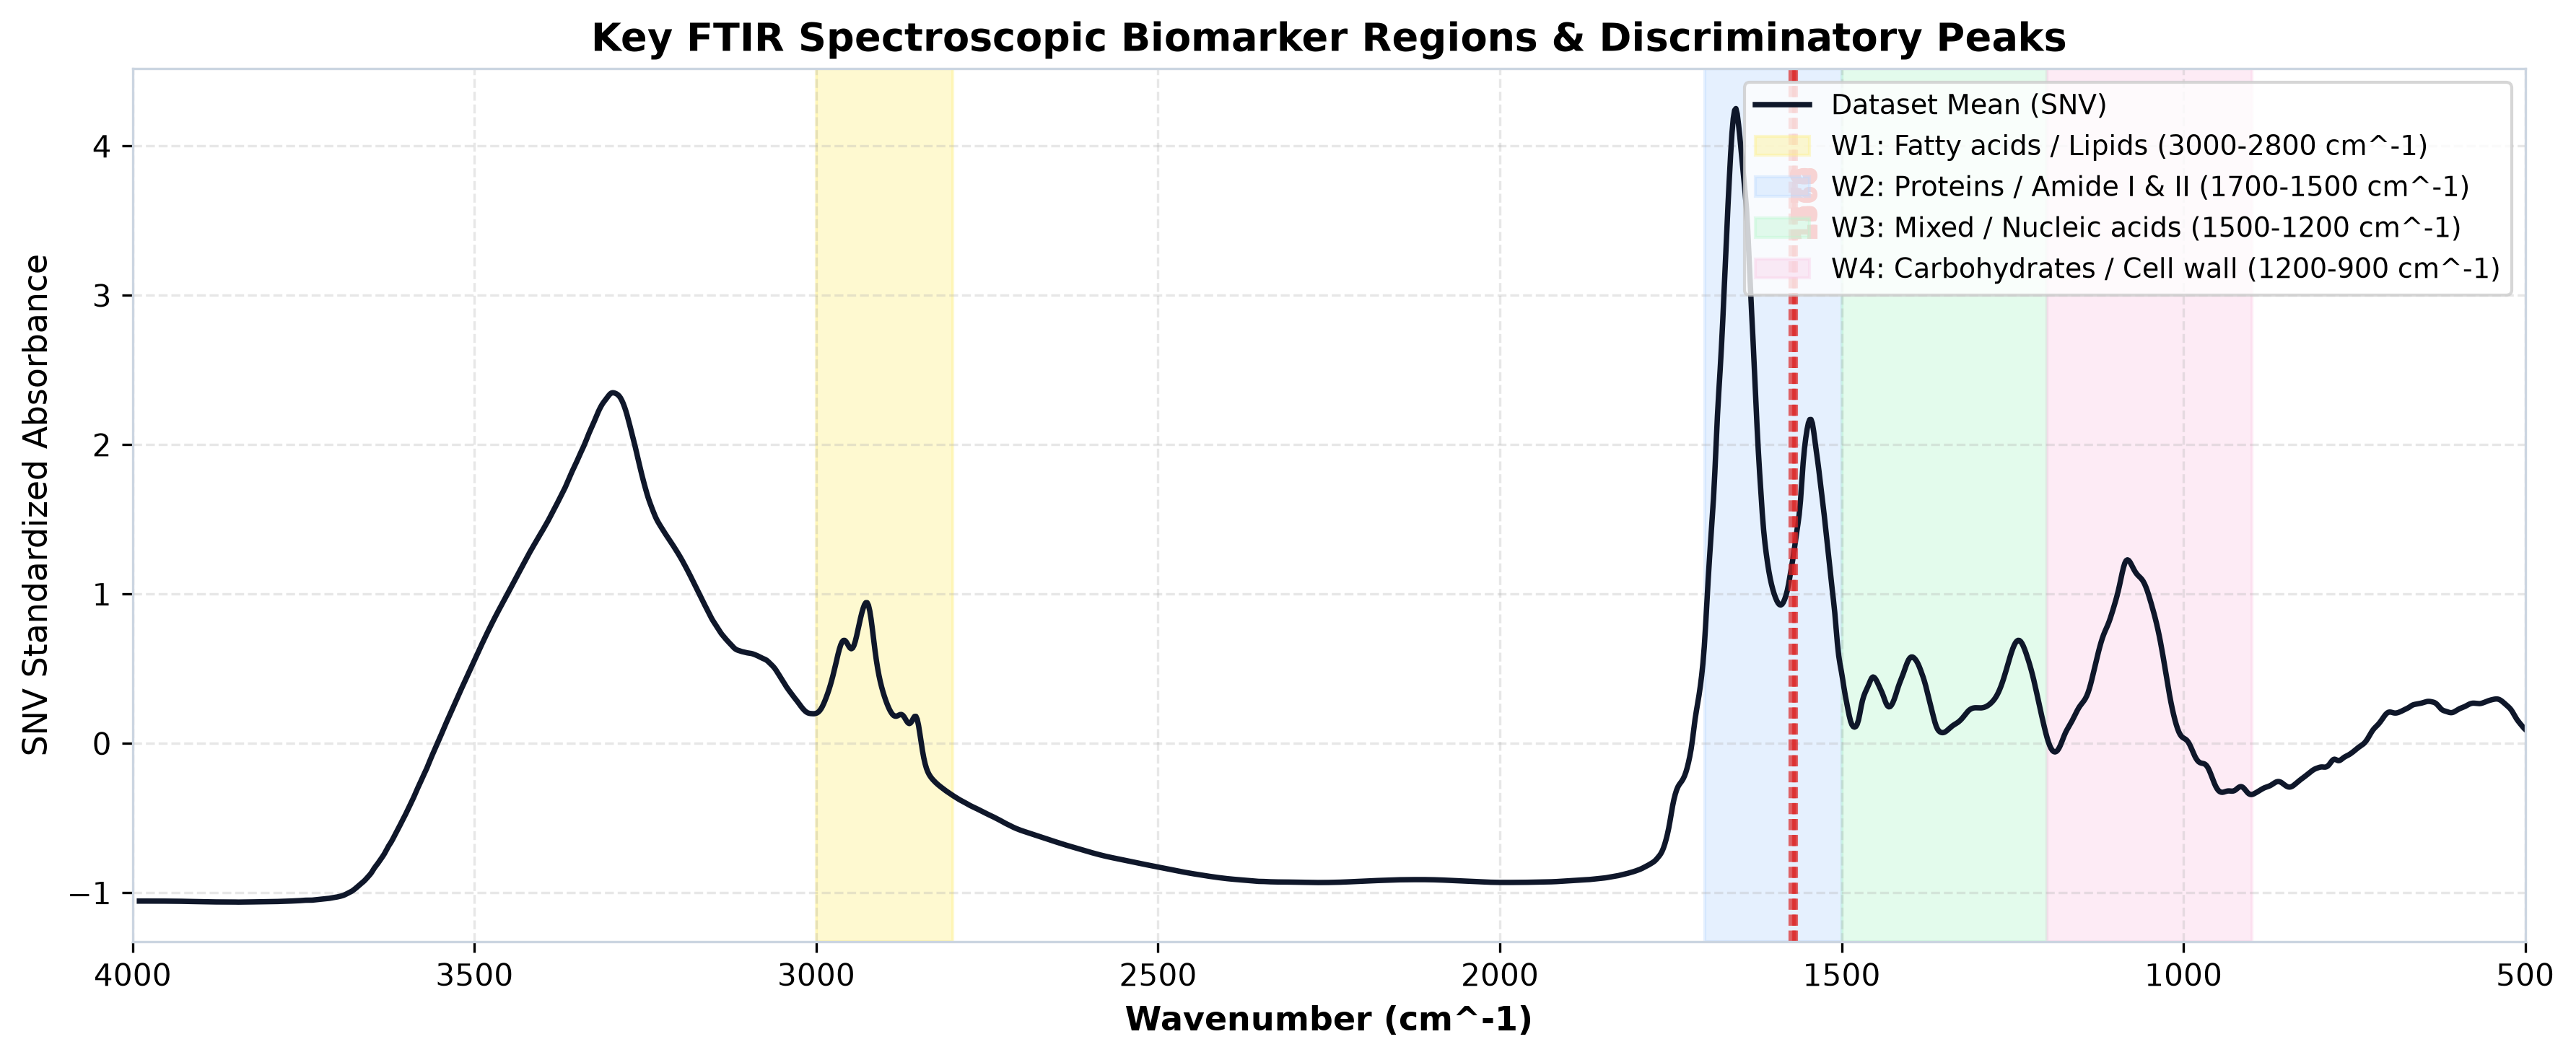
\includegraphics[width=0.9\linewidth]{output_ftir/spectral_biomarker_regions.png}
    \caption{Key FTIR spectroscopic functional group regions (W1--W4) with top discriminatory biomarker peaks identified by Random Forest feature importance.}
    \label{fig:biomarkers}
\end{figure}

\begin{figure}[H]
    \centering
    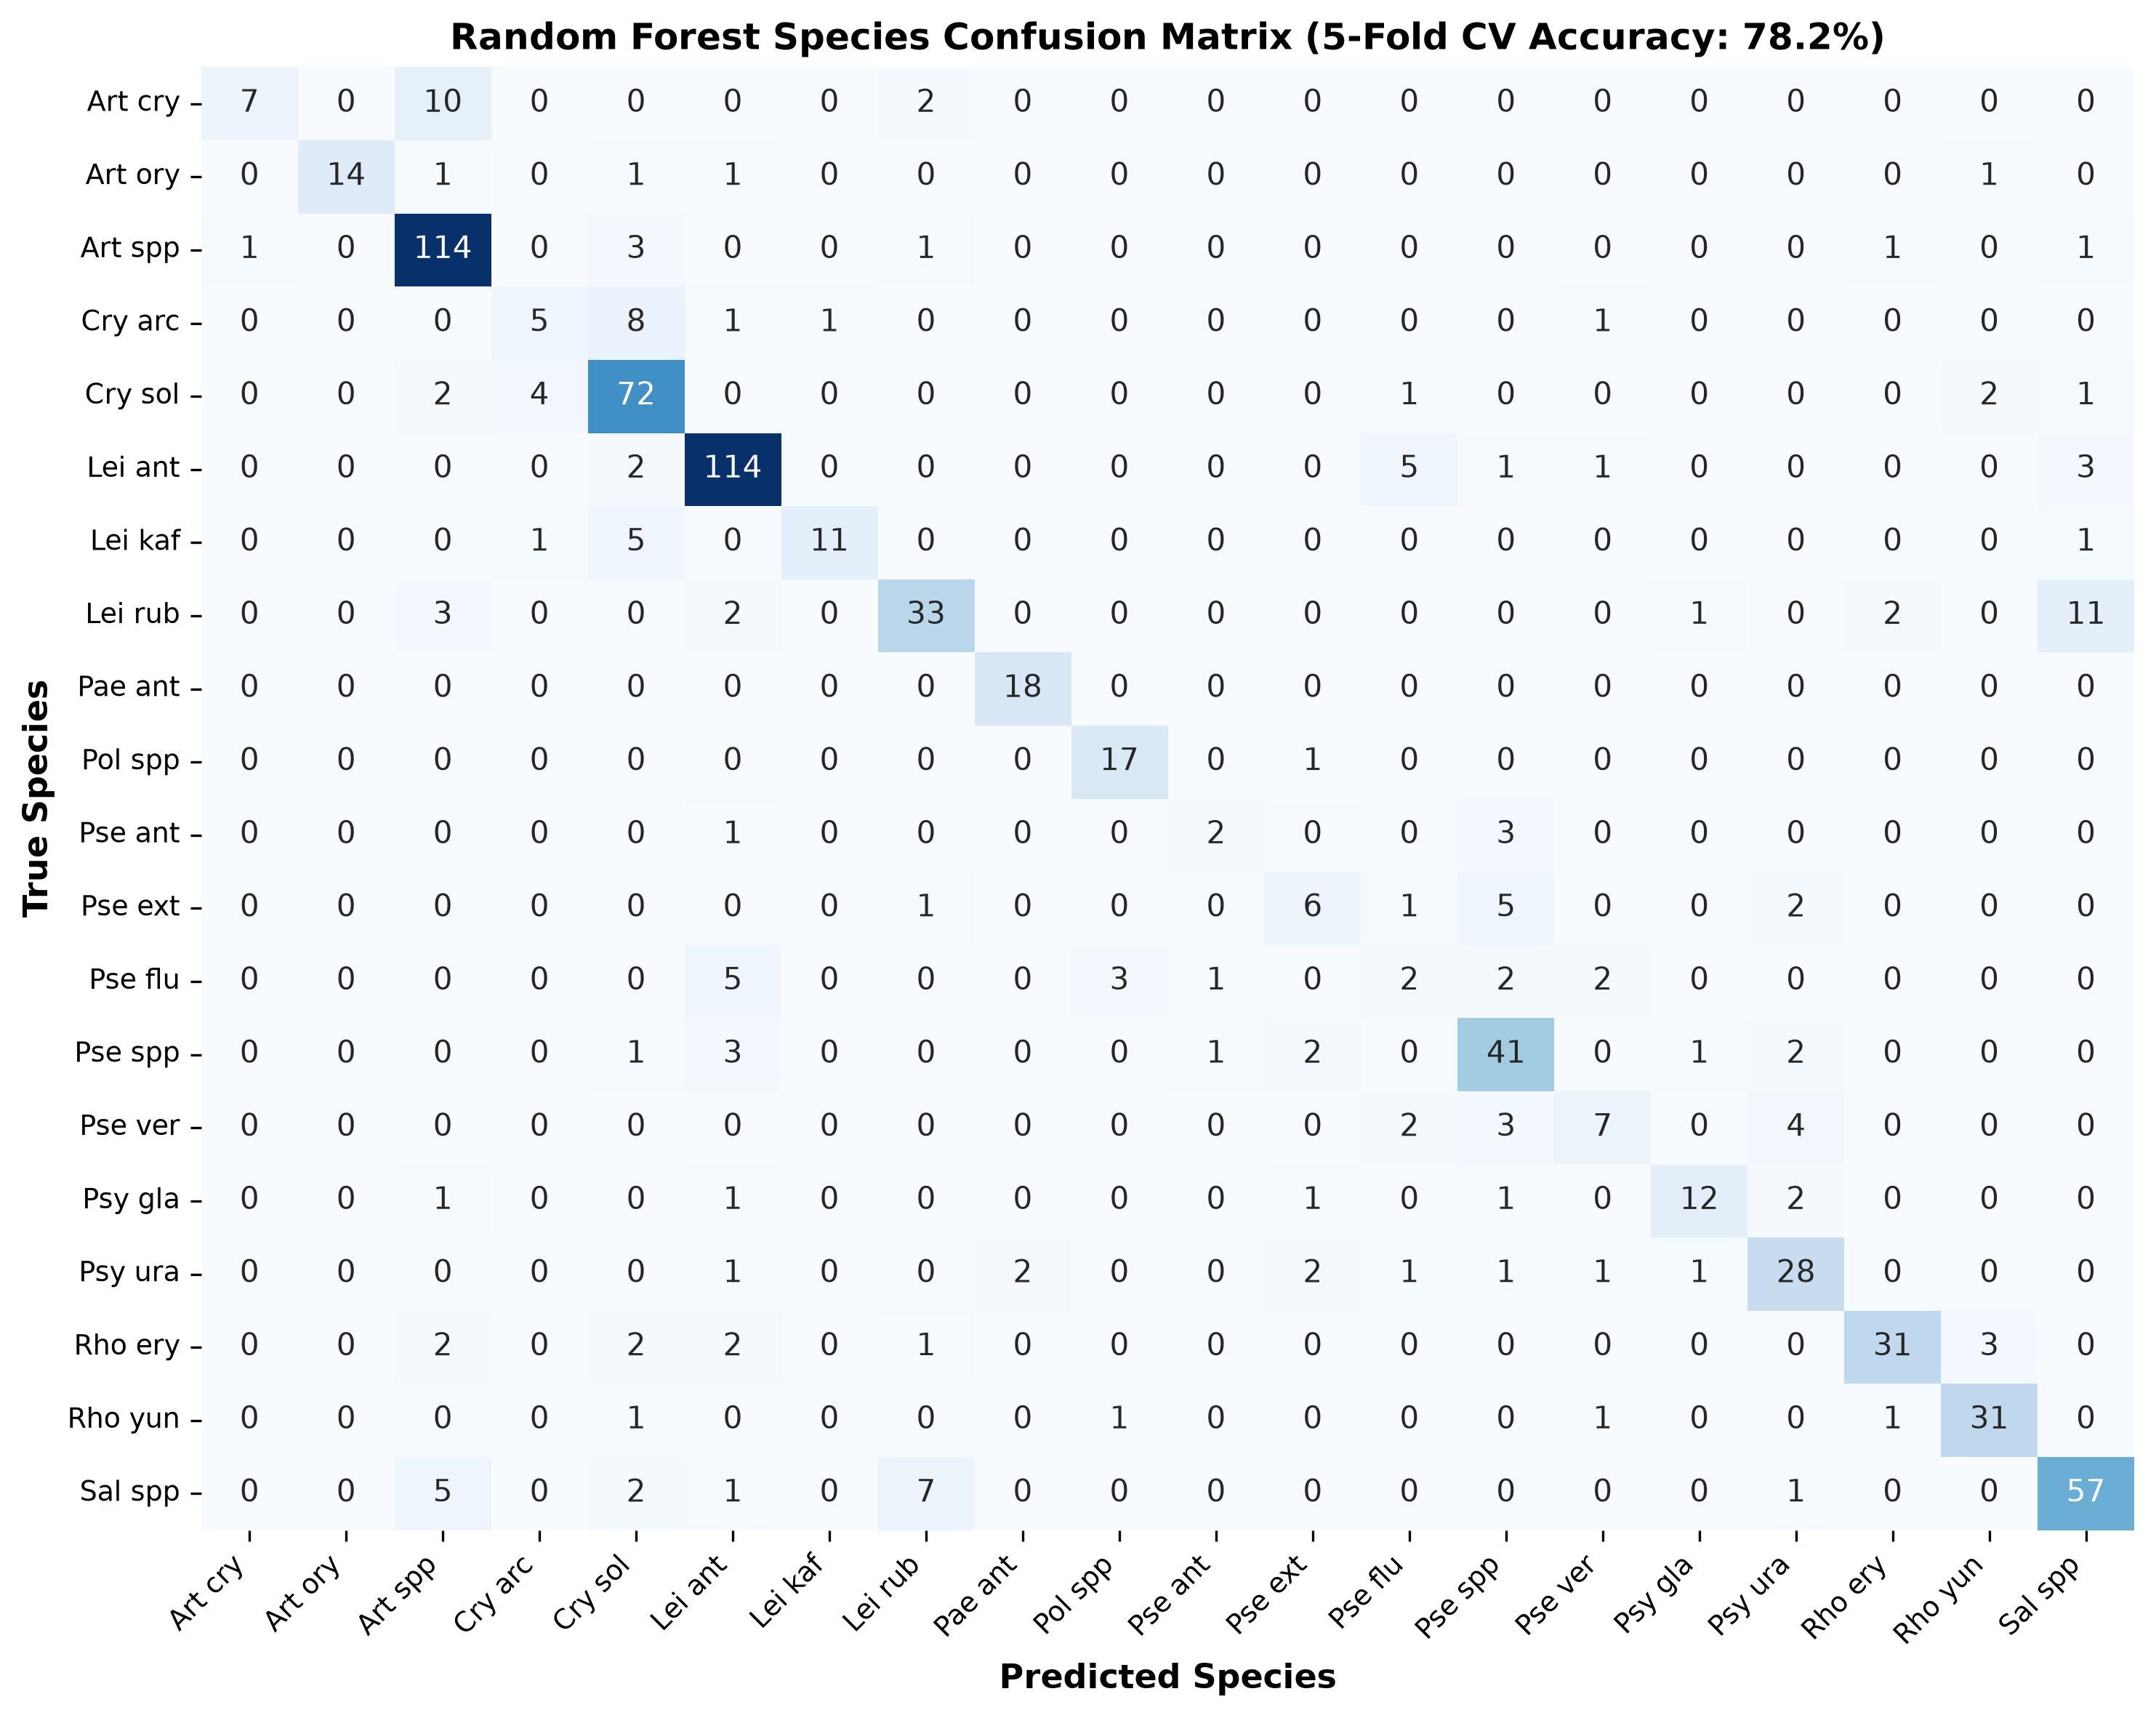
\includegraphics[width=0.75\linewidth]{output_ftir/confusion_matrix.png}
    \caption{Confusion matrix for Random Forest species-level classification across 20 bacterial taxa under 5-fold cross-validation.}
    \label{fig:cm}
\end{figure}

\section{Discussion}
The results confirm that ATR-FTIR spectroscopy provides an accurate phenotypic fingerprint capable of distinguishing 45 bacterial isolates across 20 psychrotolerant/environmental species.

The prominent role of the \textbf{Amide II region (1571--1565~cm$^{-1}$)} and \textbf{Amide I region (1687--1683~cm$^{-1}$)} as top discriminatory features underscores significant variation in cell wall-bound and cytoplasmic protein secondary structures among cold-adapted bacteria. Psychrotolerant genera such as \textit{Cryobacterium}, \textit{Leifsonia}, and \textit{Psychrobacter} modulate their proteome and membrane fluidity (reflected in the \textbf{2925~cm$^{-1}$ lipid peak}) to maintain biological function at lower temperatures (18$^\circ$C).

Furthermore, the clear differentiation between Gram-positive Actinomycetota (\textit{Arthrobacter}, \textit{Leifsonia}, \textit{Rhodococcus}) and Gram-negative Pseudomonadota (\textit{Pseudomonas}) in both PCA space and HCA dendrograms demonstrates that cell wall peptidoglycan thickness vs. lipopolysaccharide outer membrane composition imparts distinct infrared absorption signatures in the 1200--900~cm$^{-1}$ window.

Compared to traditional 16S rRNA gene sequencing---which can struggle to discriminate closely related species within genera like \textit{Arthrobacter} or \textit{Pseudomonas} due to sequence conservation---whole-cell FTIR spectroscopy measures phenotypic macromolecular expressions that reflect active metabolic adaptation.

\section{Conclusion}
This study demonstrates that ATR-FTIR spectroscopy combined with SNV preprocessing, PCA, Ward's HCA, and machine learning classifiers (SVM/Random Forest) provides a high-throughput, accurate, and cost-effective approach for bacterial strain profiling. The top discriminatory peaks identified in the Amide I/II and lipid stretching regions provide biochemical insights into cold-adapted bacterial cell wall and protein architecture.

\section*{Data Availability Statement}
All raw spectral files, preprocessed matrices, PCA coordinate scores, and trained model objects are available in the project repository:
\begin{itemize}
    \item Raw Spectral CSV: \texttt{output\_ftir/ftir\_raw\_data.csv} (795 rows $\times$ 1,820 columns)
    \item SNV Preprocessed CSV: \texttt{output\_ftir/ftir\_snv\_preprocessed.csv}
    \item PCA Scores CSV: \texttt{output\_ftir/ftir\_pca_scores.csv}
    \item Interactive Web App: \texttt{index.html} (Local server \texttt{http://localhost:8000})
\end{itemize}

\end{document}
